\documentclass[电力电子]{subfiles}
\begin{document}
\section{分析计算题}
\begin{ti}[10 分]
	在三相半波整流电路中,$\alpha = 30^\circ$,如果 $a$ 相的触发脉冲消失
	\begin{enumerate}
		\item 试绘出在电阻性负载整流电压 $u_{d}$ 的波形;
		\item 计算 $U_{d}$。
	\end{enumerate}
\end{ti}

\begin{ti}[15 分]
	三相全控桥整流电路,带阻感负载,$L$ 值极大,电阻 $R = $ \SI{5}{\Omega},变压器二次相电压为 \SI{200}{V},控制角 $\alpha = 30^\circ$,试回答:
	\begin{enumerate}
		\item 画出整流输出电压 $u_{\dd}$ 的波形,画出晶闸管 \V 的电压 $u_{\V}$ 的波形;
		\item 计算整流输出平均电压 $U_{\dd}$、$I_{\dd}$。
	\end{enumerate}
\end{ti}

\begin{ti}[15 分]
	三相全控桥整流电路,带阻感负载,$L$ 值极大,电阻 $R = $ \SI{5}{\Omega},变压器二次相电压为 \SI{200}{V},控制角 $\alpha = 90^\circ$,试回答:
	\begin{enumerate}
		\item 画出整流输出电压 $u_{\dd}$ 的波形,画出晶闸管 \V 的电压 $u_{\V}$ 的波形;
		\item 计算整流输出平均电压 $U_{\dd}$、$I_{\dd}$。
	\end{enumerate}
\end{ti}

\begin{ti}[15 分]
	三相全控桥整流电路,带阻感负载,$L$ 值极大,电阻 $R = $ \SI{5}{\Omega},变压器二次相电压为 \SI{200}{V},控制角 $\alpha = 0^\circ$,试回答:
	\begin{enumerate}
		\item 画出整流输出电压 $u_{\dd}$ 的波形,画出晶闸管 \V 的电压 $u_{\V}$ 的波形;
		\item 计算整流输出平均电压 $U_{\dd}$、$I_{\dd}$。
	\end{enumerate}
\end{ti}

\begin{ti}[15 分]
	三相全控桥整流电路,带阻感负载,$L$ 值极大,电阻 $R = \SI{5}{\Omega}$,变压器二次相电压为 \SI{100}{V},控制角 $\alpha = 60^\circ$,试回答:
	\begin{enumerate}
		\item 画出整流输出电压 $u_{\dd}$ 的波形,画出晶闸管 \V 的电压 $u_{\V}$ 的波形;
		\item 计算整流输出平均电压 $U_{\dd}$、$I_{\dd}$;
		\item 计算晶闸管电流的有效值。
	\end{enumerate}
\end{ti}

\begin{ti}[10 分]
	已知自耦变压器基本绕组为 1-0,调整绕组 1-3 与 1-2 之间的匝数是 1-0 的 \SI{10}{\percent}。试分析图示两组反并联晶闸管组成的电路,是如何实现在输入电压波动时,使输出电压 $U_{0}$ 保持稳定?
	\begin{center}
		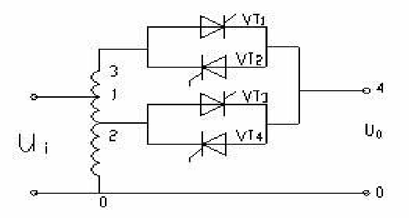
\includegraphics[scale=0.5]{figure/fig5.png}
	\end{center}
\end{ti}

\begin{ti}[10 分]
	有一单相半波相控整流电路,负载电阻 $R_{\dd} = \SI{10}{\Omega}$,直接接到交流 \SI{220}{V} 电源上,如图所示。在控制角 $\alpha = 60^\circ$ 时,求输出电压平均值 $U_{\dd}$、输出电流平均值 $I_{\dd}$,并选择晶闸管元件(考虑两倍裕量)。
\end{ti}

\begin{ti}[10 分]
	单相全控桥式整流电路接大电感负载。已知:$U_{2} = \SI{220}{V}$,$R = \SI{10}{\Omega}$,$\alpha = 60^\circ$。
	\begin{enumerate}
		\item 计算整流输出电压 $U_{\dd}$、整流输出电流的平均值 $I_{\dd}$;
		\item 计算流过晶闸管电流的有效值 $I_{\V}$;
		\item 画出输出电压 $U_{\dd}$ 的波形和流过晶闸管 \V 的电流 $i_{\V}$ 波形。
	\end{enumerate}
\end{ti}

\begin{ti}[10 分]
	有一个三相半波可控整流电路如图所示。已知带大电感负载,$\alpha = 45^\circ$,$R = \SI{2}{\Omega}$ 变压器二次相电压 $U_{2} = \SI{380}{V}$。试
	\begin{enumerate}
		\item 计算负载的平均整流电压 $U_{\dd}$ 和负载电流 $I_{\dd}$;
		\item 计算晶闸管电流的有效值 $I_{\mathrm{V}_1}$;
		\item 按裕量系数 2 确定晶闸管的额定电压。
	\end{enumerate}
\end{ti}

\begin{ti}
	单相全控桥式有源逆变电路如图示,变压器二次电压交有效值 $U_{2} = \SI{200}{V}$,回路总电阻 $R = \SI{1.2}{\Omega}$,平波电抗器 $L$ 足够大,可使负载电流连续,当 $\beta = 45^\circ$,$E_{\dd} = - \SI{188}{V}$ 时,按要求完成下列各项:
	\begin{enumerate}
		\item 画出输出电压 $U_{\dd}$ 的波形;
		\item 画出晶闸管 \V 的电流波形 $i_{\V}$;
		\item 计算输出电流平均值 $I_{\dd}$;
		\item 计算晶闸管电流的平均值 $I_{\dd \mathrm{V}_{1}}$ 和有效值 $I_{\mathrm{V}_{1}}$。
	\end{enumerate}
\end{ti}

\begin{ti}[10 分]
	如图所示降压斩波电路,已知 $E = \SI{200}{V}$,$R = \SI{10}{\Omega}$,$L$ 值极大。采用脉宽调制控制方式,当控制周期 $T = \SI{50}{\upmu s}$,全控开关 VT 的导通时间 $t_{\mathrm{on}} = \SI{20}{\upmu s}$,试完成下列各项要求。
	\begin{enumerate}
		\item 计算稳态时输出电压的平均值 $U_{\oo}$、输出电流的平均值 $I_{\oo}$;
		\item 给出 VT 导通、关断时的两种工作模式的等效电路。
	\end{enumerate}
\end{ti}

\begin{ti}[10 分]
	单相全控桥式整流电路接大电感负载。已知 $R = \SI{10}{\ohm}$,$\alpha = 45^\circ$,$U_{2} = \SI{100}{\volt}$,试回答:
	\begin{enumerate}
		\item 计算输出整流电压 $U_{\dd}$,输出电流平均值 $I_{\dd}$;
		\item 计算晶闸管电流的有效值 $I_{\mathrm{V}_{1}}$;
		\item 按裕量系数 2 确定晶闸管的额定电流。
	\end{enumerate}
\end{ti}

\begin{ti}[10 分]
	分析下图所示斩波电路的基本工作原理。形状 Q 是可以代替什么元件?
	\begin{center}
		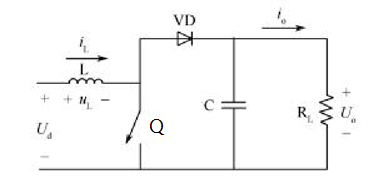
\includegraphics[width=0.5\textwidth]{figure/fig7.png}
	\end{center}
\end{ti}

\begin{ti}[10 分]
	三相桥式全控整流电路,$U_{2} = \SI{100}{V}$,带电阻电感负载,$R = \SI{5}{\ohm}$,$L$ 值极大,当 $\alpha = 60^\circ$ 时,要求:计算 $U_{\dd}$、$I_{\dd}$、$I_{\dd \mathrm{T}}$ 和 $I_{\mathrm{VT}}$ 以及变压器二次侧电流的有效值 $I_{2}$。
\end{ti}

\begin{ti}[10 分]
	已知自耦变压器基本绕组为 1-0,调整绕组 1-3 与 1-2 之间的匝数是 1-0 的 \SI{10}{\percent}。试分析图示两组反并联晶闸管组成的电路,是如何实现在输入电压波动时,使输出电压 $U_{0}$ 保持稳定?
	\begin{center}
		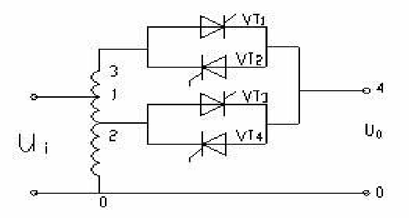
\includegraphics[scale=0.5]{figure/fig5.png}
	\end{center}
\end{ti}

\begin{ti}[10 分]
	有一个三相全控桥整流电路如图所示。已知电感负载 $L = \SI{0.2}{H}$、$\alpha = 75^\circ$、$R = \SI{1}{\ohm}$、变压器二次相电压 $U_{2} = \SI{100}{V}$。试画出 $u_{\dd}$ 的波形,计算负载的平均整流电压 $U_{\dd}$ 和负载电流平均值 $I_{\dd}$,计算变压器二次电流的有效值 $I_{2}$。
\end{ti}

\begin{ti}[10 分]
	一单相交流调压器,电源为工频 \SI{220}{V},阻感串联作为负载,其中 $R = \SI{1}{\ohm}$,$L = \SI{2}{mH}$。试求:
	\begin{enumerate}
		\item 开通角 $\alpha$ 的变化范围;
		\item 负载电流的最大有效值;
		\item 最大输出功率及此时电源侧的功率因数。
	\end{enumerate}
\end{ti}

\begin{ti}[10 分]
	下图所示的降压斩波电路中,$E = \SI{100}{V}$,$L = \SI{100}{mH}$,$R = \SI{0.5}{\ohm}$,$E_{\mathrm{M}} = \SI{10}{V}$,采用脉宽调制控制方式,$T = \SI{20}{\upmu s}$,当 $T_{\mathrm{on}} = \SI{4}{\upmu s}$ 时。求:
	\begin{enumerate}
		\item 输出电压平均值 $U_{\oo}$;
		\item 输出电流平均值 $I_{\oo}$;
		\item 并判断负载电流是否连续。
	\end{enumerate}
\end{ti}

\begin{ti}[10 分]
	下图所示的降压斩波电路中,$E = \SI{100}{V}$,$L = \SI{100}{mH}$,$R = \SI{0.5}{\ohm}$,$E_{\mathrm{M}} = \SI{10}{V}$,采用脉宽调制控制方式,$T = \SI{20}{\upmu s}$,当 $T_{\mathrm{on}} = \SI{4}{\upmu s}$ 时。求:
	\begin{enumerate}
		\item 输出电压平均值 $U_{\oo}$;
		\item 输出电流平均值 $I_{\oo}$;
		\item 并判断负载电流是否连续。
	\end{enumerate}
\end{ti}
\end{document}